% Designed Companion Part IV figure
% Intended for \input{...} beside the matching canonical problem.
\begin{figure}[ht]
\centering
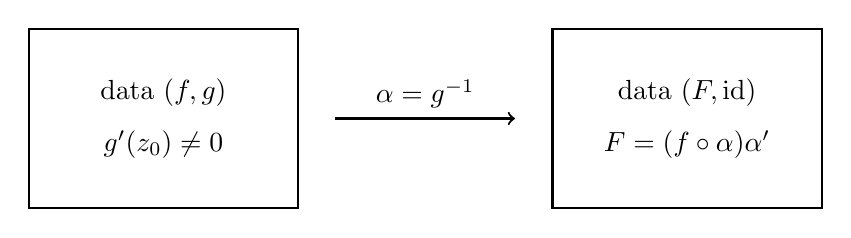
\begin{tikzpicture}[scale=0.95]
  \begin{scope}[xshift=-3.5cm]
    \draw[thick] (-1.8,-1.2) rectangle (1.8,1.2);
    \node at (0,0.35) {data $(f,g)$};
    \node at (0,-0.35) {$g'(z_0)\ne0$};
  \end{scope}
  \draw[->,thick] (-1.2,0)--(1.2,0) node[midway,above] {$\alpha=g^{-1}$};
  \begin{scope}[xshift=3.5cm]
    \draw[thick] (-1.8,-1.2) rectangle (1.8,1.2);
    \node at (0,0.35) {data $(F,\mathrm{id})$};
    \node at (0,-0.35) {$F=(f\circ\alpha)\alpha'$};
  \end{scope}
\end{tikzpicture}
\caption{At a regular point of the Gauss map, $g$ is locally invertible. Reparametrizing by $\alpha=g^{-1}$ changes the Weierstrass data to $(F,\mathrm{id})$, making the Gauss-map coordinate itself the local complex parameter.}
\label{fig:cp-iv-0082-weierstrass-gauss-coordinate}
\end{figure}
